\documentclass[a4paper,titlepage]{article}

\makeatletter
\def\input@path{{}}
\makeatother

\usepackage{Comandi}
\usepackage{Riferimenti}
\usepackage{Stile}
\usepackage{subfiles}
\usepackage[italian]{babel}


\begin{document}

\maketitle

\newpage
\tableofcontents
\listoffigures
\newpage

\section{Abstract}
Il sito è stato realizzato con l'intenzione di fornire uno strumento di supporto per il tracciamento e la gestione di Use Case e requisiti, aspetto fondamentale nella realizzazione di un prodotto software.
Nel nostro percorso universitario abbiamo affrontato il corso di Ingegneria del Software, che prevede lo svolgimento di un lavoro di gruppo, della durata di un semestre. Questo progetto, dedicato allo sviluppo di un prodotto software proposto da aziende esterne all'università di Padova, aveva anche lo scopo di farci imparare come affrontare nel miglior modo possibile un problema di discrete dimensioni, per farci maturare sia da un punto di vista delle nostre conoscenze, sia nel nostro lato umano. \\
All'inizio di questo percorso, il nostro gruppo si è reso conto della mancanza di uno strumento da utilizzare per raccogliere e poter gestire i requisiti del proponente individuati durante l'analisi del problema, e i relativi casi d'uso. \\
Il tracciamento dei requisiti è cruciale per poter controllare se tutte le richieste del cliente sono state prese in considerazione e per poter valutare, in qualsiasi momento del progetto, quali di questi requisiti vengono soddisfatti dal prodotto, e quali no. Per questo motivo il gruppo SWEgo ha deciso di creare questo sito per offrire una serie di funzionalità di fondamentale importanza nella realizzazione di un prodotto Software. \\
Ai nostri utenti diamo la possibilità di creare tutti i propri requisiti, decidendo per ognuno:
\begin{itemize}
	\item \textbf{codice};
	\item \textbf{nome};
	\item \textbf{descrizione};
	\item \textbf{tipo} (funzionale, di vincolo, di qualità o prestazionale);
	\item \textbf{importanza} (obbligatorio, desiderabile o facoltativo da implementare);
	\item \textbf{stato di soddisfacimento};
	\item \textbf{fonte};
\end{itemize}
In relazione ai requisiti possono essere tracciati anche gli Use Case. Si tratta di una tecnica usata nei processi di ingegneria del software per effettuare in maniera esaustiva e non ambigua, la raccolta dei requisiti al fine di produrre software di qualità e per valutare ognuno di essi focalizzandosi sugli attori che interagiscono col sistema. Per gli Use Case può essere specificato:
\begin{itemize}
	\item \textbf{codice};
	\item \textbf{nome};
	\item \textbf{descrizione};
	\item \textbf{scenario principale};
	\item \textbf{scenario alternativo};
	\item \textbf{padre};
	\item \textbf{estensioni};
	\item \textbf{inclusioni};
	\item \textbf{i requisti associati};
	\item \textbf{attori};
\end{itemize}


\newpage
\section{Utenti destinatari}
Il sito è rivolto in particolare agli studenti universitari che devono affrontare un progetto simile a quello di Ingegneria del Software dell'Università di Padova, ma questo non vieta l'utilizzo di SWEgo a coloro inizino lo sviluppo di un prodotto software, in ambito lavorativo o in qualsiasi altro contesto. \\
SWEgo inoltre dà la possibilità a tutti i suoi utenti di comunicare con noi sviluppatori, tramite le nostre pagine social o via e-mail, per proporre miglioramenti, nuove idee, consigli e feedback, utili a far crescere il nostro prodotto e proporlo a nuove categorie di utenti destinatari.
\newpage
\section{Accessibilità}
\subsection{Separazione tra struttura, presentazione e comportamento}
Per migliorare l'accesso al sito a qualsiasi categoria di utenti è stata mantenuta la separazione tra struttura, presentazione e comportamento. \\
La prima è stata sviluppata tramite documenti HTML5. Questi richiamano i fogli di stile esterni CSS, che implementano la presentazione, e gli script esterni di JavaScript che ne determinano il comportamento.
\subsection{Tag meta}
Per ogni pagina web sono stati inseriti i seguenti tag meta:
\begin{itemize}
	\item \textbf{title}: titolo;
	\item \textbf{description}: descrizione sintetica;
	\item \textbf{keywords}: lista di parole chiave che permette di specificare gli argomenti trattati;
	\item \textbf{author}: indica gli autori della pagina;
	\item \textbf{viewport}: utilizzato per "comunicare" al browser come adattare il sito per dispositivi con diverse misure.
\end{itemize}


\subsection{Percepibilità}
La percepibilità consiste in: 
	\begin{itemize}
		\item fornire alternative testuali per qualsiasi contenuto non testuale, in modo che questo possa essere trasformato in altre forme fruibili secondo le necessità degli utenti;
		\item rendere più semplice agli utenti la visione dei contenuti.
	\end{itemize}
	In particolare il gruppo ha seguito queste regole:
	\begin{itemize}
		\item attributo \textit{alt} con un appropriato testo sostitutivo a tutte le immagini;
		\item non sono state utilizzate immagini per riportare il testo, rendendo il contenuto informativo accessibile anche agli utenti che utilizzano gli screen reader;
		\item attributo \textit{scope= "col"} per specificare la cella header di una colonna, o gruppo di colonne in una tabella(sempre rivolto agli utenti che utilizzano gli screen reader);
		\item un tag \textit{label} che descrive la finalità di ogni textfield di ogni form;
		\item un tag \textit{legend} per tutti i fieldset, utile a descriverne il contenuto.
	\end{itemize}
\subsubsection{Colori}
Per rendere il più semplice possibile agli utenti la visione dei contenuti è stato adottato un appropriato schema di colori, il quale garantisce un certo contrasto cromatico.
	In particolare, miriamo a dare meno disagi possibili agli utenti affetti da particolari patologie agli occhi, quali deuteranopia, protanopia e tritanopia. \\
	Gli screenshot qui sotto sono una simulazione di come un utente appartenente a questa categoria vede il nostro sito.\\
	\begin{figure}
	\centering
		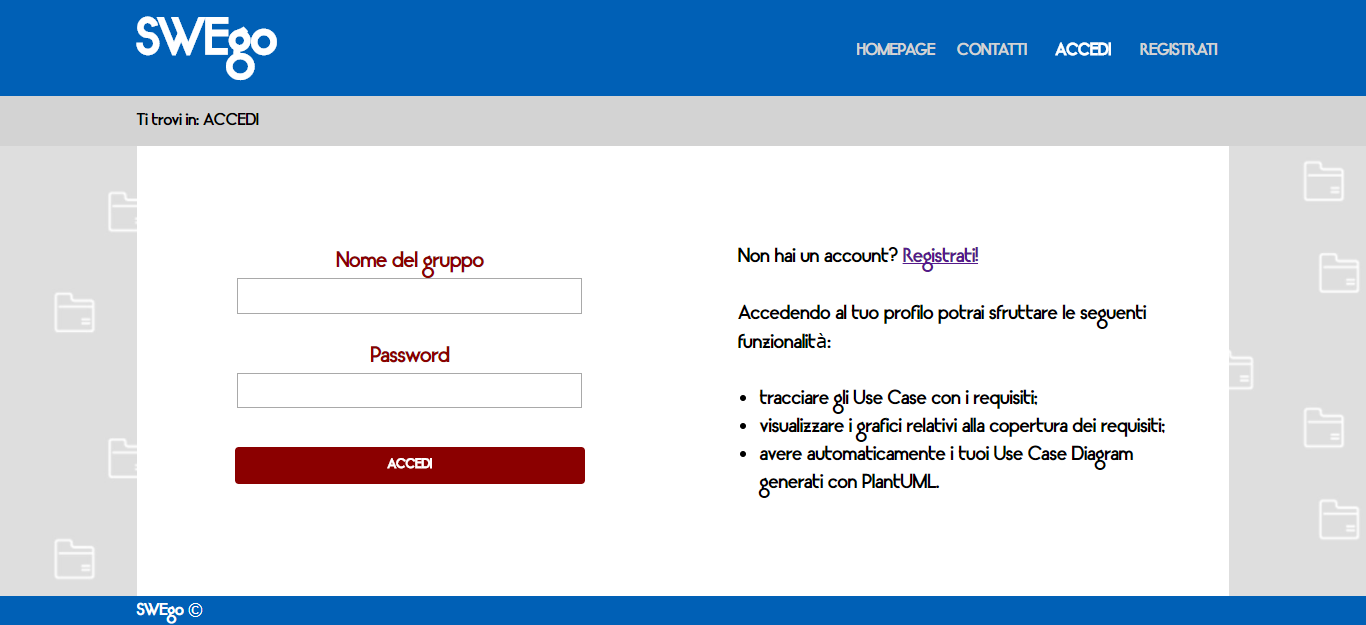
\includegraphics[scale=0.4]{img/normale.png}\\[1cm] \caption{Pagina di login vista da un utente normale.}
	\end{figure}
	\begin{figure}
	\centering
		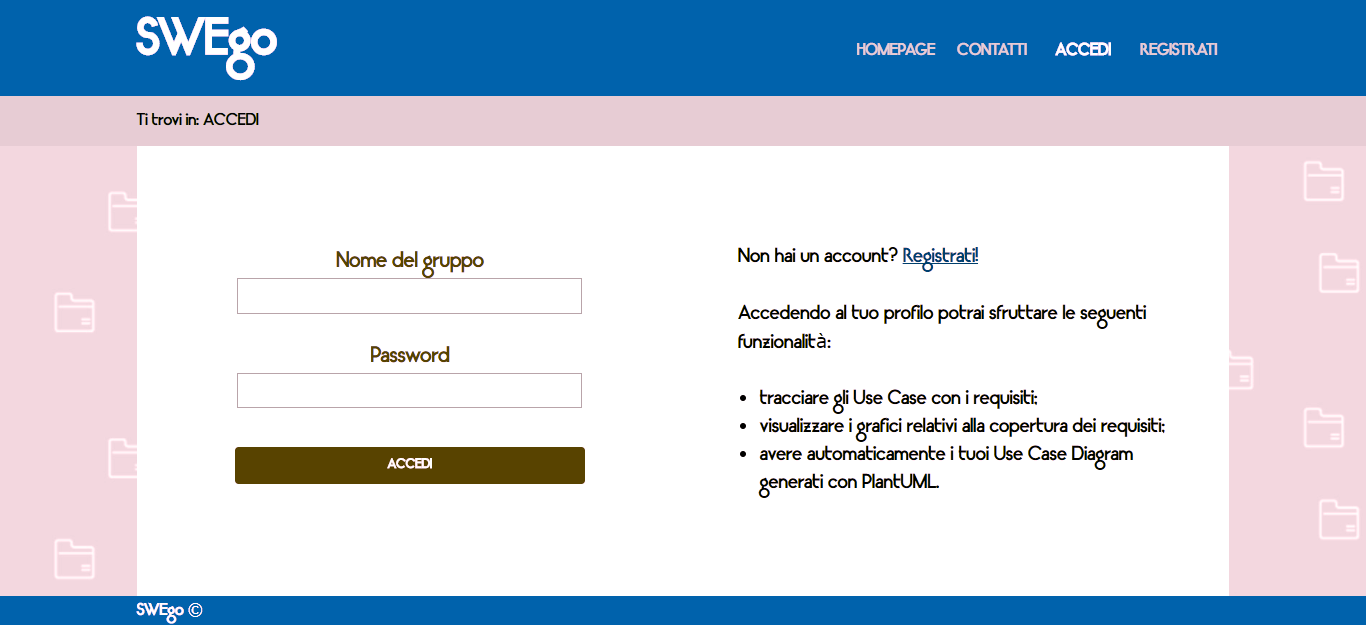
\includegraphics[scale=0.3]{img/deuteranopia.png}\\[1cm] \caption{Pagina di login vista da un utente affetto da deuteranopia}
	\end{figure}
	\begin{figure}
	\centering
		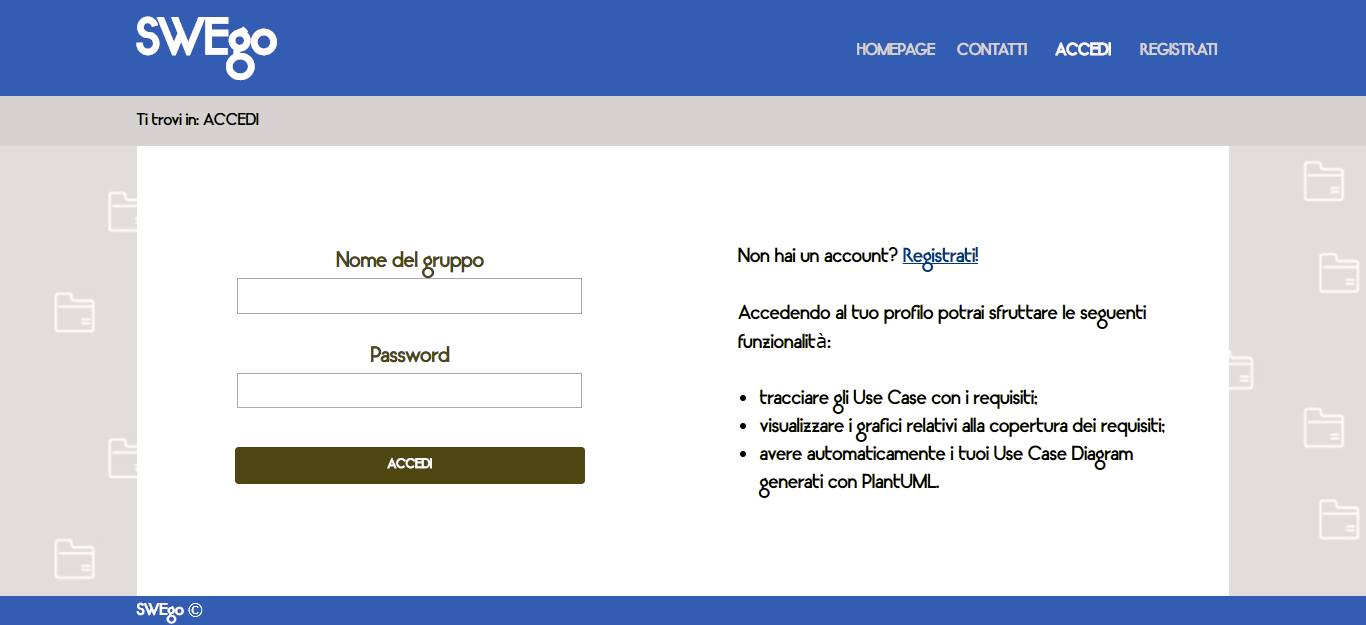
\includegraphics[scale=0.3]{img/protanopia.png}\\[1cm] \caption{Pagina di login vista da un utente affetto da protanopia}
	\end{figure}
	\begin{figure}
	\centering
		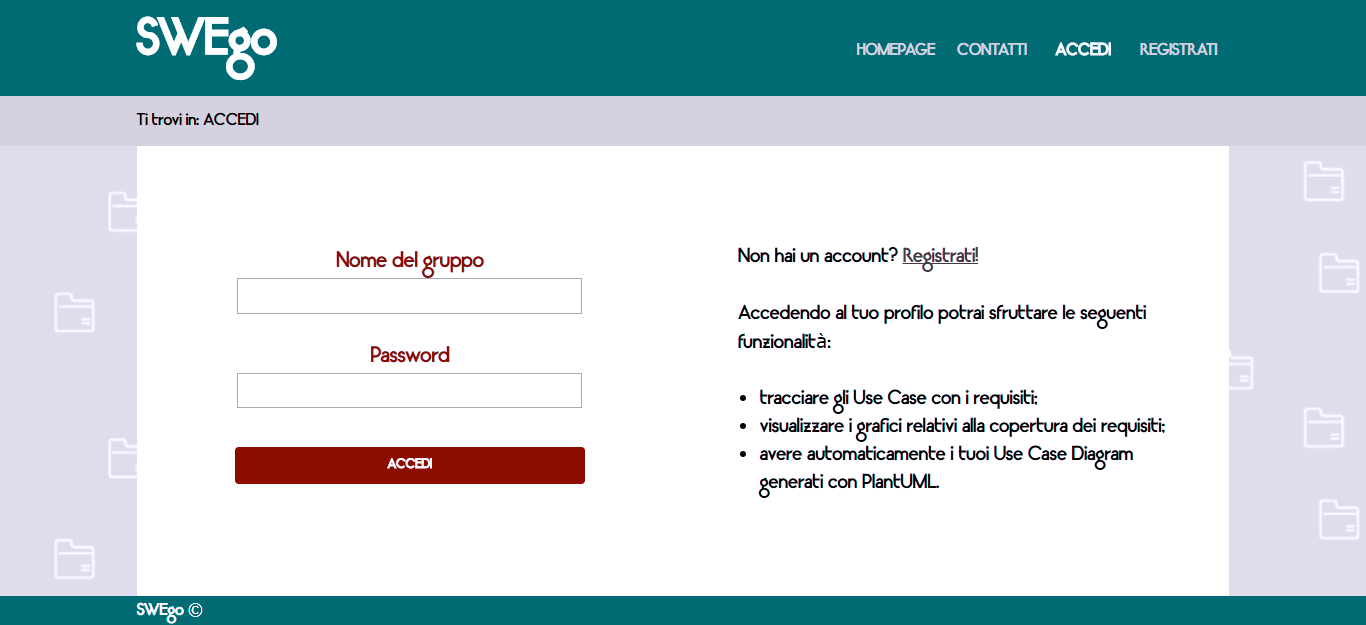
\includegraphics[scale=0.3]{img/tritanopia.png}\\[1cm] \caption{Pagina di login vista da un utente affetto da tritanopia}
	\end{figure}
		\begin{figure}
	\centering
		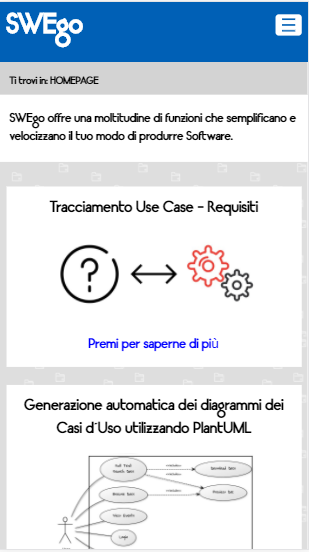
\includegraphics[scale=0.8]{img/normale_mobile.jpeg}\\[1cm] \caption{Pagina mobile di login vista da un utente normale.}
	\end{figure}
	\begin{figure}
	\centering
		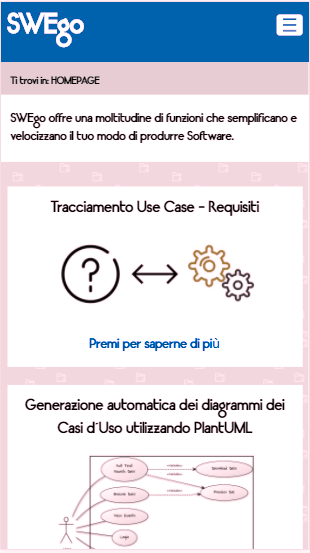
\includegraphics[scale=0.8]{img/deuteranopia_mobile.png}\\[1cm] \caption{Pagina mobile di login vista da un utente affetto da deuteranopia}
	\end{figure}
	\begin{figure}
	\centering
		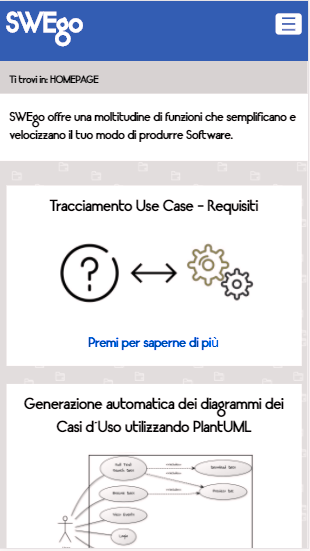
\includegraphics[scale=0.8]{img/protanopia_mobile.png}\\[1cm] \caption{Pagina mobile di login vista da un utente affetto da protanopia}
	\end{figure}
	\begin{figure}
	\centering
		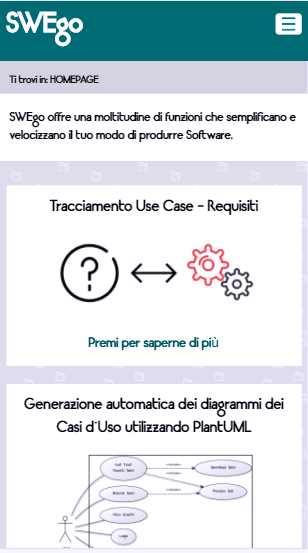
\includegraphics[scale=0.8]{img/tritanopia_mobile.png}\\[1cm] \caption{Pagina mobile di login vista da un utente affetto da tritanopia}
	\end{figure}
	\newpage
\subsection{Usabilità}
Al fine di migliorare l'esperienza d'uso degli utenti sono state inserite le seguenti facilitazioni:
\begin{itemize}
	\item \textbf{tabindex}: non è stato ridefinito il comportamento del pulsante tab tramite l'attributo tabindex, in quanto il gruppo ritiene quello di default agevole per la navigazione;
	\item \textbf{link per spostarsi al contenuto}: prima della barra di navigazione è stato inserito un link nascosto per saltarla, permettendo agli utenti che utilizzano uno screen reader di passare direttamente al contenuto;
	\item 
\end{itemize}
Inoltre per rendere ben navigabile il sito si è fatto uso di:
\begin{itemize}
	\item \textbf{breadcrumb} che permette di capire in che pagina ci si trova;
	\item \textbf{mappa del sito}.
\end{itemize}

\subsection{Comprensibilità}
Le informazioni del sito devono risultare comprensibili per gli utenti. A tal scopo si è fatto utilizzo di:
	\begin{itemize}
		\item \textit{xml:lang=en} per specificare che alcune parole sono inglesi;
		\item menù quasi uguali per tutte le pagine, rendendo la voce di menù della pagina attuale non cliccabile;
		\item apposite label e istruzioni che aiutano l'utente a inserire dati corretti;
		\item un gruppo di \textit{checkbox} al posto di \textit{<select multiple>}, in quanto risulta molto più comprensibile e di più facile utilizzo.
	\end{itemize}
\subsection{Robustezza}
Il gruppo si è prefisso come scopo la più alta compatibilità possibile tra browser, rendendo il sito utilizzabile fino a Internet Explorer 8. Questo è stato reso possibile facendo utilizzo di regole CSS e funzioni JavaScript compatibili
con quest'ultimo. \\
Inoltre il sito è stato testato in diversi altri browser (Google Chrome 59.0, Mozilla Firefox 53.0 e Microsoft Edge), dove l'aspetto e le funzionalità rimangono pressoché inalterate.

\subsection{Screen Reader}
Per testare la compatibilità del sito con uno Screen Reader, è stato scelto di usare il programma gratuito NVDA. Alcuni membri del gruppo hanno utilizzato tale programma per navigare all’interno del sito, sia nell’area utente sia nell’area di amministrazione, senza riscontrare particolari problemi. Il sito risulta quindi utilizzabile anche da parte di una persona che non può usare un browser canonico, ma deve fare affidamento ad uno screen reader.
\newpage
\section{Struttura}
\subsection{Struttura del sito}
Il sito è diviso in diverse aree, raggiungibili tramite il menù, a seconda se l'utente è un utente loggato, non loggato o un admin. In particolare:
\begin{itemize}
	\item \textbf{Utente non loggato}
	\begin{itemize}
		\item \textbf{Homepage}: è la homepage del sito dove si può vedere una panoramica delle funzionalità offerte;
		\item \textbf{Accedi/Registrati}: in queste pagine l'utente può accedere al sito con il proprio profilo oppure crearne uno nuovo se non si è mai registrato;
		\item \textbf{Contatti}: in questa pagina vengono mostrate le pagine social e la mail attraverso le quali è possibile contattare gli sviluppatori, o semplicemente rimanere informati sulle novità di SWEgo.
	\end{itemize}
	\item \textbf{Utente loggato}:
	\begin{itemize}
		\item \textbf{Homepage} (come sopra);
		\item \textbf{Contatti} (come sopra);
		\item \textbf{Attori}: in questa pagina si trova il riepilogo degli attori inseriti dall'utente. Un attore può essere inteso come un ruolo coperto da un certo insieme di entità interagenti col sistema (inclusi utenti umani, altri sistemi software, dispositivi hardware e così via). E' possibile aggiungere, eliminare o modificare tutti gli attori;
		\item \textbf{Use Case}: in questa pagina si trovano tutti gli Use Case inseriti dall'utente, con la possibilità di inserirne di nuovi ed eliminare o modificare quelli già presenti;
		\item \textbf{Fonti}: in questa pagina l'utente può visualizzare le fonti inserite nel sistema; una fonte può essere intesa come il soggetto dal quale un requisito è stato estrapolato;
		\item \textbf{Requisiti} (come per gli Use Case, con al posto i requisiti);
		\item \textbf{Tracciamento}: in questa pagina si può vedere un riassunto dei requisiti associati ad ogni Use Case;
		\item \textbf{Profilo}: in questa pagina l'utente può visualizzare e modificare i propri dati, visualizzare alcuni grafici riassuntivi e generare le immagini degli Use Case tramite plantIml;
	\end{itemize}
	\item \textbf{Admin} (oltre alle pagine da utente loggato):
	\begin{itemize}
		\item \textbf{Summary}: MANCA
	\end{itemize}
Da ogni pagina è raggiungibile la \textit{mappa del sito}(diversa in base alla tipologia dell'utente) attraverso il link presente nel footer.
\end{itemize}
\subsection{Struttura delle pagine}
Ogni pagina del sito è differente per i contenuti ma vi sono alcuni elementi che ricorrono in ognuna di esse:
\begin{itemize}
	\item \textbf{header}: contiene il logo del sito e i link alle pagine precedentemente descritte per ogni categoria di utente;
	\item \textbf{breadcrumb}: fa sapere all'utente in che pagina si trova in quel momento descrivendo anche il percorso seguito per arrivarci;
	\item \textbf{footer}: contiene un riferimento al gruppo, un link alla mappa del sito e le immagini che certificano che le pagine sono conformi a HTML5 e CSS3.
\end{itemize}
\newpage
\section{Presentazione}
Per la rappresentazione dell'interfaccia grafica del sito si è rispettato lo standard CSS3.\\
L'uso di specifiche proprietà del CSS3 sono state limitate al minimo in modo da essere il più possibile compatibile con versioni di browser meno recenti e permettere un degrado elegante anche in caso non siano supportate.
Per garantire una buona usabilità del sito i colori per la realizzazione del sito sono stati scelti in modo da avere un buon contrasto tra testo e sfondo, in questo modo sono facilmente visibili anche da utenti affetti da particolari
difetti visivi come daltonismo.\\
Abbiamo prestato attenzione a non avere elementi lampeggianti nel sito per non creare disagi ad utenti affetti da epilessia fotosensibile.

\subsection{Divisione dei file}
Il sito non presenta problemi nel ridimensionamento della pagina grazie all'utilizzo di fogli di stile diversi a seconda della dimensione del dispositivo. In particolare nella cartella css sono presenti 3 file:
\begin{itemize} 
	\item \textbf{desktop.css}: contiene le regole di stile per dispositivi con una "width" maggiore a 520px; 
	\item \textbf{mobile.css}: contiene le regole di stile per dispositivi mobile con "width" minore o uguale a 520px;
	\item \textbf{print.css}: contiene le regole di stile relative alla stampa delle varie pagine del sito.
\end{itemize}
Le differenze tra versione desktop e mobile sono ristrette al diverso posizionamento di alcuni elementi delle pagine, mantenendo così uno stile grafico del sito omogeneo, in questo modo per l'utente abituato ad accedere alla
versione desktop non si ritrova confuso da un sito completamente diverso. \\
In particolare nella versione mobile le voci del menù possono essere visualizzate attraverso un apposito pulsante, che nella versione desktop viene nascosto, per ridurre lo spazio occupato dall'header.
\newpage
\section{Comportamento}
La parte relativa al comportamento delle pagine è stata gestita con JavaScript. In particolare si è fatto uso dei seguenti script:
\begin{itemize}
	\item \textbf{features.js}: ha il compito di far comparire o nascondere la descrizione dei vari div presenti nella homepage del sito, cliccando l'apposito link;
	\item \textbf{nav.js}: ha il compito di far comparire o nascondere il menù del sito nella versione mobile, cliccando l'apposito pulsante;
	\item \textbf{requirement.js}: ha il compito di filtrare la tabella dei requisiti, in base a quanto l'utente scrive nell'apposito input per la ricerca. I requisiti vengono selezionati solo se il codice o il nome corrispondono all'input dell'utente. Se la ricerca non da risultati, viene mostrata una descrizione appropriata;
	\item \textbf{useCase.js}: stesso compito di "requirement.js" per la tabella degli Use Case (il filtro qui viene applicato su codice e nome).
	\item \textbf{user.js}: ha il compito di costruire i grafici e far comparire o nascondere il form del cambio password e i grafici stessi nella pagine del profilo utente.
\end{itemize}
\newpage
\section{Link}
Nella realizzazione del sito sono state tenute in considerazione le consuetudini per i link, ossia tenere il testo sottolineato per indicare la presenza di un link e cambiarne il colore una volta visitato. In alcuni casi è stato deciso di non rispettare tali pratiche, in particolare:
\begin{itemize}
	\item nei link del menù, poiché gli utenti sono ormai abituati ad utilizzare menù con link visitati e non visitati indistinti. Inoltre, è molto probabile che i link nel menù principale diventino tutti visitati dopo un beve periodo di utilizzo del sito, rendendo quindi superflua la distinzione;
	\item nei link del breadcrumb, per lo stesso motivo dei link del menù;
	\item nelle pagine index e user dove sono presenti dei link per nascondere o mostrare del contenuto della pagina;
	\item nel footer il colore del link per la mappa del sito è grigio per non essere confuso con il colore dello sfondo.
\end{itemize}

\newpage
\section{PHP}

\begin{itemize}
	\item \textbf{index.php}: è la pagina iniziale del sito che ne mostra le funzionalità. E' una pagina dinamica in quanto le voci del menu cambiano se l'utente è loggato o meno;
	\item \textbf{login.php}: è la pagina per accedere al sito con il proprio profilo attraverso il nome del gruppo e la propria password. Nel caso il login fallisca viene mostrato un messaggio d'errore;
	\item \textbf{logout.php}: ha il compito di distruggere la sessione;
	\item \textbf{registration.php}: è la pagina per creare un proprio profilo all'interno del sito. Nel form SCRIVERE DEI CONTROLLI
	\item \textbf{contacts.php}: mostra le pagine social e la mail per rimanere in contatto e informati con SWEgo. E' una pagina dinamica per lo stesso motivo di index.php;
	\item \textbf{tracking.php}: mostra il tracciamento tra Use Case e requisiti del progetto creato dall'utente loggato in quel momento;
	\item \textbf{user.php}: è la pagina del profilo dell'utente dove può visualizzare tutti suoi dati; in particolare l'utente loggato può creare dei grafici a torta, attraverso l'apposito link, che mostrano il riassunto dei requisiti obbligatori, desiderabili e facoltativi soddisfatti in quel determinato momento. Da questa pagina è possibile anche creare le immagini degli Use Case attraverso PlantUml e fare il logout dal proprio profilo;
	\item \textbf{viewRequirement.php, viewTracking.php, viewUsecase.php}: sono le pagine che rispettivamente recuperano e mostrano i dati relativi ai requisiti, Use Case e tracciamento Use Case-requisiti del progetto dell'utente;
	\item \textbf{insertActor.php, insertSource.php}: sono le pagine che recuperano e mostrano le informazioni degli attori e delle fonti del progetto dell'utente; danno anche la possibilità di inserirne di nuovi attraverso l'apposito form;
	\item \textbf{insertRequirement.php, insertUseCase}: sono le pagine che danno la possibilità di inserire nuovi requisiti e Use Case nel progetto;
	\item \textbf{deleteX.php}: sono le pagine che danno la possibilità di eliminare dal progetto, e quindi dal database, attori, fonti, requisiti, Use Case e il tracciamento Use Case/requisiti creati precedentemente dall'utente; 
	\item \textbf{modifyX.php}: stesso comportamento di deleteX.php, ma in questo caso queste pagine danno la possibilità di modificare i dati precedentemente inseriti.
\end{itemize}

AGGIUNGEREI I CONTROLLI FATTI SUI FORM MA NON LI SO SCRIVERE BENE
\newpage
\section{Test}
\subsection{Validazione}
Per la validazione, è stato usato il validatore online messo a disposizione da W3C. Per validare ogni pagina, si sono seguiti i seguenti passi:
\begin{itemize}
	\item esecuzione del file nel browser;
	\item copia del codice sorgente;
	\item controllo con il validatore tramite "validate by input".
\end{itemize}
Tutte le pagine e i file CSS hanno superato questo test.
\subsection{Browser}
Senza riscontrare grosse differenze, il sito è stato testato sui seguenti browser:
\begin{itemize}
	\item Mozilla Firefox 53.0;
	\item Google Chrome 59.0;
	\item Internet Explorer 8, 9 , 10, 11;
	\item Microsoft Edge.
\end{itemize}
\subsubsection{JavaScript}
Nel caso in cui JavaScript risulti disattivato non viene rilevato alcun tipo di errore, e il sito può garantire la maggior parte delle sue funzionalità. In particolare resta possibile visualizzare, inserire, modificare ed eliminare tutti i dati del progetto, ma non ricercare requisiti o Use Case tramite l'apposito input di ricerca.

\newpage
\section{Ruoli}
Il gruppo ha deciso di assegnare diversi compiti tra i vari membri, anche se le decisioni più importanti sono state prese insieme. In particolare:
\begin{itemize}
	\item \textbf{Marco Bonolo}: realizzazione della parte back-end del progetto;
	\item \textbf{Nicola Tintorri}: creazione di alcune pagine HTML e CSS mobile di tutte le pagine, e alcuni script JS;
	\item \textbf{Mauro Carlin}: creazione di alcune pagine HTML con relativo CSS desktop, print e script JS;
	\item \textbf{Luca Bertolini}: creazione di alcune pagine HTML con relativo CSS desktop, print e script JS.
\end{itemize}


\end{document}
